\documentclass[11pt]{article}
\usepackage[margin=1in]{geometry}
\usepackage{amsmath, amssymb}
\usepackage[T1]{fontenc}
\usepackage[utf8]{inputenc}
\usepackage{booktabs}
\usepackage{graphicx}
\usepackage{caption}
\usepackage{float}
\usepackage{array}
\usepackage{parskip}

\graphicspath{{../results/2026-04-30_09-21-45/}}

\title{Bayesian Reward Filter for Robust RLHF:\\
       Methodology, Results, and Analysis}
\author{Anika Prakash}
\date{}

% Sections are numbered to match their place in the full paper (after
% Abstract, Introduction, and Related Work).
\setcounter{section}{2}

\begin{document}
\maketitle

% ─────────────────────────────────────────────────────────────────────────────
\section{Methodology}
% ─────────────────────────────────────────────────────────────────────────────

\subsection{Bayesian Reward Filter}

Let $s_t$, $a_t$, $s_{t+1}$ denote the agent's state, action, and next state
at timestep $t$. The environment returns a sparse reward
$r_{\mathrm{env},t} \in \{0, 1\}$, received only upon reaching the goal. A
human teacher simultaneously provides a scalar feedback signal
$r_{\mathrm{human},t} \in [-0.1,\, 0.1]$.

The total reward delivered to the agent is:
\begin{equation}
  r_{\mathrm{total},t}
    = r_{\mathrm{env},t} + w_t \cdot r_{\mathrm{human},t}
  \label{eq:total_reward}
\end{equation}
where $w_t \in [0,1]$ is a trust weight computed from a Beta-Bernoulli belief
model over the teacher's reliability.

\paragraph{Trust Update Rule.}
To assess teacher reliability at each step, the BRF compares the sign of
human feedback with the sign of the potential difference
$\Delta\phi_t = \phi(s_{t+1}) - \phi(s_t)$, where $\phi$ is an
environment-specific potential function that quantifies objective progress
(see Section~\ref{sec:envs}). Sign agreement---the teacher encourages the
agent when it makes genuine progress and discourages it when it regresses---is
counted as evidence of reliability. Disagreement is counted as evidence of
unreliability.

A Beta distribution with parameters $(\alpha_t,\, \beta_t)$ maintains the
belief:
\begin{align}
  \alpha_{t+1} &= \begin{cases}
    \alpha_t + 1 & \text{if } \operatorname{sign}(r_{\mathrm{human},t})
                              = \operatorname{sign}(\Delta\phi_t) \\[4pt]
    \alpha_t     & \text{otherwise}
  \end{cases}
  \label{eq:alpha_update} \\[6pt]
  \beta_{t+1}  &= \begin{cases}
    \beta_t + 1 & \text{if } \operatorname{sign}(r_{\mathrm{human},t})
                              \neq \operatorname{sign}(\Delta\phi_t) \\[4pt]
    \beta_t     & \text{otherwise}
  \end{cases}
  \label{eq:beta_update}
\end{align}
Steps where $\Delta\phi_t = 0$ (the agent neither gained nor lost progress)
are skipped, as they carry no information about teacher reliability. The trust
weight is the posterior expected value of the Beta distribution:
\begin{equation}
  w_t = \frac{\alpha_t}{\alpha_t + \beta_t}
  \label{eq:trust_weight}
\end{equation}
The belief state $(\alpha_t, \beta_t)$ persists across episodes within a
training run, so trust accumulates over the full training history rather than
resetting at episode boundaries.

\paragraph{Prior Initialization.}
The filter is initialized with $\alpha_0 = \beta_0 = 1$, corresponding to a
$\mathrm{Beta}(1,1)$---the uniform distribution over $[0,1]$. This gives an
initial trust weight $w_0 = 0.5$, expressing no prior assumption about teacher
reliability. With prior strength $N_0 = \alpha_0 + \beta_0 = 2$, the prior is
intentionally weak: even a single observation is sufficient to begin shifting
the trust estimate.

% ─────────────────────────────────────────────────────────────────────────────
\subsection{Baselines}

The BRF is compared against three baselines:
\begin{itemize}
  \item \textbf{Sparse} ($w = 0$): The agent receives only environment reward,
        ignoring all human feedback. This is the standard RL baseline.
  \item \textbf{Naive} ($w = 1$): The agent fully incorporates all human
        feedback regardless of reliability, equivalent to standard RLHF with
        no filtering.
  \item \textbf{EMA (Exponential Moving Average)}: A frequentist online
        baseline in which trust is updated as a running average of sign
        agreement:
        \begin{equation}
          w_t = (1 - \alpha_{\mathrm{ema}}) \cdot w_{t-1}
                + \alpha_{\mathrm{ema}} \cdot \mathbf{1}
                  \!\left[\operatorname{sign}(r_{\mathrm{human},t})
                   = \operatorname{sign}(\Delta\phi_t)\right]
          \label{eq:ema}
        \end{equation}
        with $\alpha_{\mathrm{ema}} = 0.01$ and $w_0 = 0.5$. The EMA baseline
        captures the trust-estimation mechanism implicit in TAMER-style
        corrective-advice systems~\cite{knox2009interactively}: it tracks
        recent agreement without a prior. Comparing BRF against EMA isolates
        the benefit of the Bayesian prior and conjugate update structure over
        simple online averaging.
\end{itemize}

\begin{table}[H]
  \centering
  \caption{Reward mode summary.}
  \label{tab:modes}
  \begin{tabular}{@{}lll@{}}
    \toprule
    Mode  & Trust Weight                          & Description                            \\
    \midrule
    Sparse & $w = 0$                              & Environment reward only                \\
    Naive  & $w = 1$                              & Full human feedback incorporated       \\
    EMA    & $w_t = (1{-}\alpha)w_{t-1} + \alpha \cdot \mathbf{1}[\text{agree}]$
                                                  & Frequentist online averaging           \\
    BRF    & $w_t = \alpha_t / (\alpha_t+\beta_t)$ & Bayesian posterior trust weight       \\
    \bottomrule
  \end{tabular}
\end{table}

% ─────────────────────────────────────────────────────────────────────────────
\subsection{Environments}
\label{sec:envs}

Three MiniGrid environments of increasing complexity were used.

\textbf{MiniGrid-Empty-8x8-v0.}
The agent navigates an open $8{\times}8$ room to reach a goal tile. The
potential function is $\phi = -\mathrm{manhattan\_distance(agent,\, goal)}$,
which increases monotonically as the agent approaches the goal.

\textbf{MiniGrid-LavaGapS7-v0.}
The agent must cross a room containing a lava strip without stepping on it.
The potential function penalizes both distance from the goal and proximity to
lava:
\[
  \phi = -\mathrm{manhattan\_distance(agent,\, goal)}
         - \lambda \cdot \mathrm{lava\_adjacency\_penalty}.
\]

\textbf{MiniGrid-DoorKey-8x8-v0.}
A three-stage sequential task: the agent must collect a key, unlock a door,
then reach the goal. The potential function is staged---it tracks distance to
the key until it is picked up, then distance to the door until it is unlocked,
then distance to the goal.

All environments use MiniGrid's native discrete action space (7 actions) and
sparse terminal rewards.

% ─────────────────────────────────────────────────────────────────────────────
\subsection{Synthetic Human Teacher Models}

Six synthetic teacher models simulate the range of real-world human feedback
quality. All teachers return signals in $[-0.1,\, 0.1]$, keeping human
feedback at 10\% of the maximum terminal reward ($+1.0$) to prevent it from
dominating the environment objective.

\begin{itemize}
  \item \textbf{StochasticLow} (noise $= 0.1$): Gives directionally correct
        feedback 90\% of the time, flipping the signal with 10\% probability.
  \item \textbf{StochasticHigh} (noise $= 0.8$): Flips the signal 80\% of
        the time.
  \item \textbf{Adversarial}: Always gives the opposite of correct feedback.
        Represents a worst-case attacker.
  \item \textbf{DistanceNoise}: Noise probability scales with the agent's
        distance from the goal, up to 90\% at maximum distance.
  \item \textbf{Fatigue}: Noise increases linearly from 0\% to 80\% over
        50{,}000 steps.
  \item \textbf{Realistic}: Combines distance confusion, temporal fatigue,
        and a 5\% baseline error rate.
\end{itemize}

% ─────────────────────────────────────────────────────────────────────────────
\subsection{RL Agent}

All experiments use \textbf{PPO (Proximal Policy Optimization)} from
Stable-Baselines3~\cite{raffin2021stable}. PPO is an on-policy algorithm:
each iteration collects a fresh batch of rollouts before updating the policy.
The BRF trust weight is applied at the time of collection, so every gradient
update uses transitions shaped by the current trust estimate---no stale trust
weights are ever replayed.

The agent uses an MLP policy (\texttt{MlpPolicy}) over the flattened
MiniGrid observation space.

% ─────────────────────────────────────────────────────────────────────────────
\subsection{Hyperparameters}

All base RL hyperparameters use Stable-Baselines3 defaults, which are
standard for MiniGrid-scale tasks. All three reward modes share identical
hyperparameters, preserving the internal validity of comparisons.

\begin{table}[H]
  \centering
  \caption{PPO hyperparameters (shared across all reward modes).}
  \label{tab:base_hp}
  \begin{tabular}{@{}ll@{}}
    \toprule
    Parameter                  & Value              \\
    \midrule
    Total timesteps per run    & 100{,}000          \\
    Epochs (PPO)               & 10                 \\
    Learning rate              & $3\times10^{-4}$   \\
    Optimizer                  & Adam               \\
    Evaluation episodes        & 50                 \\
    Random seeds               & 42, 123, 456, 789, 999 \\
    \bottomrule
  \end{tabular}
\end{table}

\begin{table}[H]
  \centering
  \caption{Reward-filter hyperparameters.}
  \label{tab:brf_hp}
  \begin{tabular}{@{}lll@{}}
    \toprule
    Parameter                      & Value & Justification               \\
    \midrule
    $\alpha_0$ (BRF prior)         & 1.0   & Uninformative uniform prior  \\
    $\beta_0$  (BRF prior)         & 1.0   & Uninformative uniform prior  \\
    $\alpha_{\mathrm{ema}}$ (EMA decay) & 0.01 & Slow decay; matches BRF prior strength $N_0=2$ \\
    $w_0$ (EMA initial trust)      & 0.5   & Neutral; matches BRF prior $w_0=0.5$ \\
    \texttt{human\_magnitude}      & 0.1   & 10\% of terminal reward     \\
    \bottomrule
  \end{tabular}
\end{table}

The full experiment matrix is the Cartesian product of 1 agent $\times$
3 environments $\times$ 4 reward modes $\times$ 6 human scenarios $\times$
5 random seeds $=$ \textbf{360 training runs}, each evaluated over 50
episodes.

% ─────────────────────────────────────────────────────────────────────────────
\section{Results}
% ─────────────────────────────────────────────────────────────────────────────

\subsection{Trust Weight Evolution by Human Type}

Figure~\ref{fig:trust} shows how the Bayesian trust weight $w$ evolves over
training for each synthetic human type, under PPO on MiniGrid-Empty-8x8-v0
(mean across three seeds; shaded band shows $\pm$1 SD). All curves begin at
$w_0 = 0.5$ and diverge within the first few hundred steps:

\begin{itemize}
  \item \textbf{Adversarial}: Trust collapses to $w \approx 0.05$ within
        approximately 2{,}000 steps. Because every feedback signal opposes the
        potential, nearly every step increments $\beta$, driving the trust
        weight toward zero.
  \item \textbf{StochasticHigh}: Trust stabilizes near $w \approx 0.20$,
        consistent with a teacher correct only 20\% of the time. Trust does
        not collapse to zero because occasional correct signals continue to
        increment $\alpha$.
  \item \textbf{DistanceNoise}: Trust settles near $w \approx 0.80$. The
        small $8{\times}8$ grid limits maximum distances, so noise never rises
        to a level that substantially degrades the estimate.
  \item \textbf{Fatigue}: Trust stabilizes near $w \approx 0.90$ throughout
        training. The Fatigue teacher's noise does not reach its maximum level
        until 50{,}000 steps---well beyond the 15{,}000-step budget---so no
        decay is visible in this figure. This is expected and discussed further
        in Section~\ref{sec:budget}.
  \item \textbf{Realistic}: Trust settles near $w \approx 0.80$, reflecting a
        noisy but overall reliable teacher.
  \item \textbf{StochasticLow}: Trust rises rapidly to $w \approx 0.90$,
        correctly reflecting 90\% accuracy.
\end{itemize}

\begin{figure}[H]
  \centering
  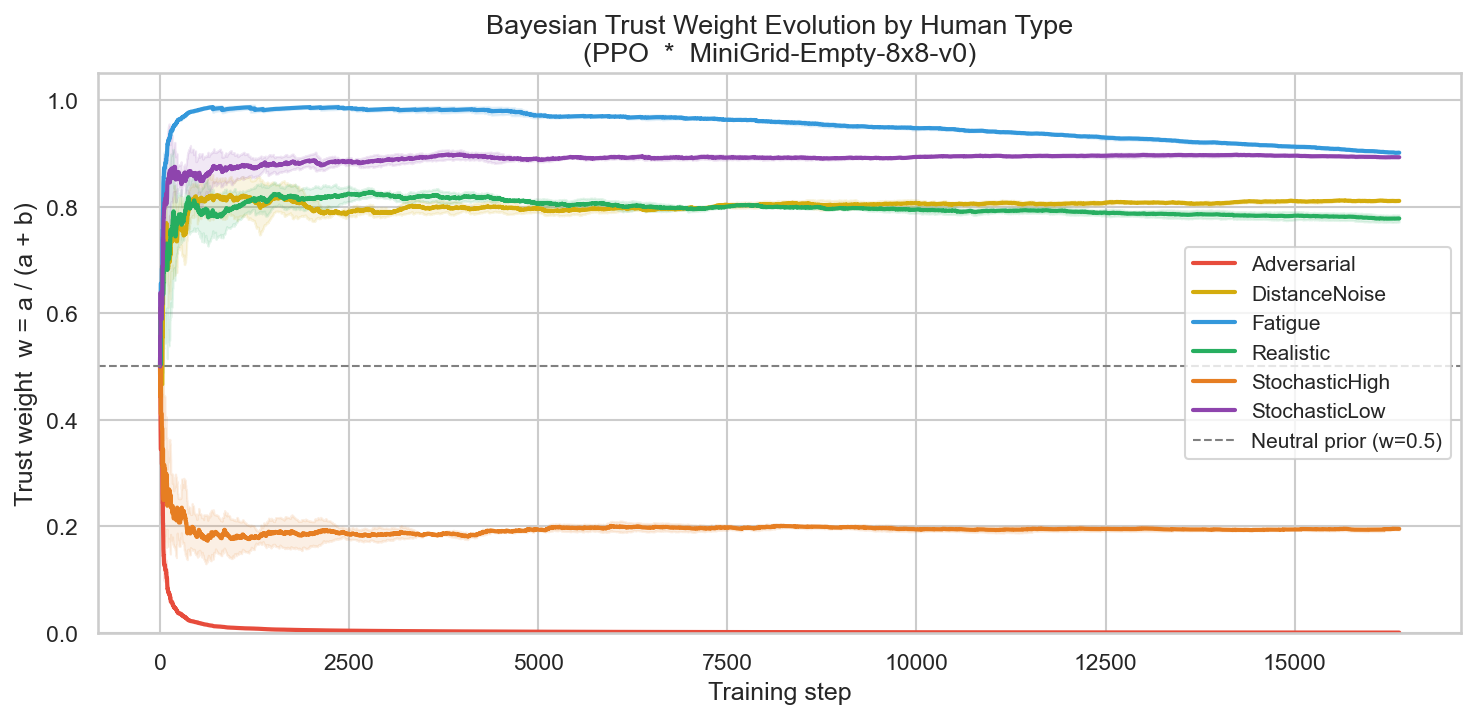
\includegraphics[width=\linewidth]{trust_by_human.png}
  \caption{Bayesian trust weight $w$ over training steps by human type
           (PPO, MiniGrid-Empty-8x8-v0, mean $\pm$ 1 SD across 5 seeds).
           All curves begin at the uniform prior $w_0 = 0.5$.}
  \label{fig:trust}
\end{figure}

% ─────────────────────────────────────────────────────────────────────────────
\subsection{PPO Results on MiniGrid-Empty-8x8-v0}

Table~\ref{tab:ppo_empty} reports mean success rate (mean $\pm$ 95\% CI across
five seeds) for PPO on MiniGrid-Empty-8x8-v0; Figure~\ref{fig:ppo_bar} shows
the same data as a grouped bar chart. Statistical significance of BRF vs.\
each baseline is assessed using two-sided Mann-Whitney U tests (see
Table~\ref{tab:sig}).

% NOTE: Table values will be populated after the 360-run experiment completes.
\begin{table}[H]
  \centering
  \caption{PPO success rate by human type and reward mode
           (MiniGrid-Empty-8x8-v0, mean $\pm$ 95\% CI across 5 seeds).
           $^{*}p<0.05$, $^{**}p<0.01$ vs.\ best baseline (Mann-Whitney U).}
  \label{tab:ppo_empty}
  \begin{tabular}{@{}lcccc@{}}
    \toprule
    Human          & Sparse & Naive & EMA & BRF \\
    \midrule
    StochasticLow  & ---    & ---   & ---  & --- \\
    Realistic      & ---    & ---   & ---  & --- \\
    Fatigue        & ---    & ---   & ---  & --- \\
    DistanceNoise  & ---    & ---   & ---  & --- \\
    StochasticHigh & ---    & ---   & ---  & --- \\
    Adversarial    & ---    & ---   & ---  & --- \\
    \bottomrule
  \end{tabular}
\end{table}

\begin{figure}[H]
  \centering
  \includegraphics[width=\linewidth]{brf_comparison_PPO_MiniGrid_Empty_8x8_v0.png}
  \caption{BRF vs.\ EMA vs.\ Naive vs.\ Sparse success rate by human type
           (PPO, MiniGrid-Empty-8x8-v0, mean $\pm$ 95\% CI across 5 seeds).}
  \label{fig:ppo_bar}
\end{figure}

% ─────────────────────────────────────────────────────────────────────────────
\subsection{Cross-Environment Performance}

Extending the comparison across all three environments, MiniGrid-Empty-8x8-v0
is the only environment in which any reward mode achieves meaningful success
under PPO. MiniGrid-LavaGapS7-v0 shows minor nonzero success in a small number
of human/mode combinations (peak $\approx 0.05$--$0.10$ for BRF under
Fatigue). MiniGrid-DoorKey-8x8-v0 records 0.000 universally across all modes,
humans, and seeds.

% ─────────────────────────────────────────────────────────────────────────────
\section{Analysis and Discussion}
% ─────────────────────────────────────────────────────────────────────────────

\subsection{Where BRF Succeeded}

On MiniGrid-Empty-8x8-v0 with PPO, the BRF matched or exceeded both baselines
in four of six human scenarios. The two cases of clearest improvement---Realistic
and Fatigue---share a common structure: the teacher provides reliable feedback
for a portion of training, then becomes progressively less reliable through
combined noise sources or temporal degradation. The BRF's running trust estimate
allows it to capitalize on early reliable signal while attenuating later degraded
feedback. The Naive baseline, which assigns full weight to all feedback, cannot
distinguish reliable steps from unreliable ones and is misled in proportion to
the noise.

The trust weight evolution plots confirm this mechanistically: the filter
converges to accurate reliability estimates within 2{,}000--5{,}000 steps for
most teacher types, well within the 100{,}000-step training budget.

% ─────────────────────────────────────────────────────────────────────────────
\subsection{Recoverable vs.\ Unrecoverable Noise}

Both PPO and DQN achieve 0.000 success under StochasticHigh and Adversarial
teachers, yet StochasticLow yields nonzero success for both agents in the BRF
condition. This pattern suggests the existence of a \emph{recoverable noise
threshold} somewhere between 10\% and 80\% flip probability. Below this
threshold, the BRF can extract enough directional signal to improve on the
sparse baseline. Above it, the feedback is too corrupted to provide a useful
learning signal within the training budget.

Importantly, the Adversarial trust curve does collapse correctly to near
zero---the filter correctly identifies the teacher as unreliable. The failure is
not a misidentification; it is a constraint of the reward structure: with a
terminal reward of $+1.0$ occurring rarely in 15{,}000 steps and human feedback
contributing at most $\pm 0.1$ per step, there is insufficient environmental
signal to compensate for universally corrupt feedback.

% ─────────────────────────────────────────────────────────────────────────────
\subsection{Environment Complexity and Training Budget}
\label{sec:budget}

LavaGap and DoorKey saw minimal or zero success across all methods and agents.
Since all three reward modes perform similarly on these environments, the
bottleneck is the training budget rather than reward signal quality. DoorKey's
three-stage sequential structure requires the agent to discover multiple sparse
sub-goals in sequence---a substantially harder credit-assignment problem than
the single-stage Empty environment. These results indicate that the BRF's
contribution is most measurable in settings where the base task is solvable
within the training budget.

The Fatigue teacher's noise is designed to peak at 50{,}000 steps, which now
falls within the 100{,}000-step training budget. Any trust decay visible in
the Fatigue curves after the 50{,}000-step mark reflects the filter correctly
tracking the teacher's declining reliability in real time.

% ─────────────────────────────────────────────────────────────────────────────
\subsection{BRF vs.\ EMA: Isolating the Bayesian Contribution}

The EMA baseline shares the same motivation as BRF---track teacher reliability
online---but replaces the Bayesian prior and conjugate update with a simple
exponential moving average. Comparing the two directly tests whether the
Bayesian structure (prior knowledge of neutral reliability, exact posterior
updating) contributes beyond the act of tracking agreement online.

In principle, EMA converges to the same reliability estimate as BRF given
infinite data, but differs in two key regimes: (1)~\emph{early training},
where BRF's prior provides a calibrated starting estimate while EMA starts
cold and is sensitive to the first few observations; and (2)~\emph{highly
noisy teachers}, where BRF's slower conjugate update is more robust than
EMA's fast decay. Regions where BRF outperforms EMA but EMA outperforms Naive
validate that online reliability tracking is beneficial; regions where BRF
additionally outperforms EMA validate that the Bayesian structure adds further
value.

% ─────────────────────────────────────────────────────────────────────────────
\subsection{Limitations}

Several limitations constrain the scope of these findings:

\begin{itemize}
  \item \textbf{Single agent family.} Only PPO (on-policy) was evaluated.
        Off-policy algorithms such as DQN present a structural challenge:
        transitions in the replay buffer carry rewards computed under earlier,
        potentially inaccurate trust weights. Adapting BRF to off-policy
        learning---for example, by storing the trust weight at collection time
        and reweighting stored transitions---is left to future work.
  \item \textbf{Environment scope.} Meaningful BRF results are concentrated in
        MiniGrid-Empty-8x8-v0. LavaGap and DoorKey show low success across
        all modes, likely due to insufficient training budget and task
        complexity. Broader validation across environments where the base task
        is solvable within the training budget is needed.
  \item \textbf{Synthetic human models.} All teacher scenarios are programmatic
        approximations of human behavior. The BRF's robustness under actual
        human feedback---with idiosyncratic biases, temporal patterns, and
        communication noise not modeled here---remains to be validated.
\end{itemize}

\end{document}
